\documentclass[aspectratio=169]{beamer}
\usetheme{Warsaw}
\usecolortheme{uiowa}
\useoutertheme[subsection=true]{smoothbars}
\usepackage{amsmath,amssymb}
\usepackage{pgfplots}
\pgfplotsset{compat=1.18}
\input{custom.tex}

\title[STAT 2020 Week 7 \hfill \insertframenumber/\inserttotalframenumber]{STAT 2020 Discussion Slides}
\subtitle{Week 7: Poisson, Integration, and Continuous Distributions}
\author{Shuo Li}
\institute{University of Iowa}
\date{\today}
\logo{
\includegraphics[width=0.12\textwidth]{iowa-logo.png}}

\begin{document}

\begin{frame}
  \titlepage
\end{frame}

\begin{frame}{Index (Outline)}
  \tableofcontents[hideallsubsections]
\end{frame}

% ==============================
\section{Week 7 Goals}
% ==============================

\subsection{Agenda}
\begin{frame}{Agenda}
  \begin{itemize}
    \item Poisson means under different time intervals and regions
    \item Quick review of integration methods
    \item One continuous piecewise example:
    \begin{itemize}
      \item CDF from PDF
      \item PDF from CDF
      \item \(\Ex(X)\) and \(\Var(X)\)
    \end{itemize}
    \item Extra practice problems (quick drills)
    \item Reminder on exam-question policy
    \item Attendance check (mental math)
  \end{itemize}
\end{frame}

% ==============================
\section{Poisson Rate and Window Size}
% ==============================

\subsection{Poisson Distribution Formula}
\begin{frame}{Poisson Distribution Formula}
  If \(X\sim\Pois(\mu)\), then
  \[
    P(X=k)=\frac{e^{-\mu}\mu^k}{k!},\qquad k=0,1,2,\dots
  \]
  In rate form:
  \[
    X=N_t\sim\Pois(\lambda t)\quad\Longrightarrow\quad
    P(N_t=k)=\frac{e^{-\lambda t}(\lambda t)^k}{k!}.
  \]
\end{frame}

\subsection{Time-Interval Example}
\begin{frame}{Poisson: Time-Interval Example}
  Assume arrivals follow \(N_t \sim \Pois(\lambda t)\).\\[4pt]
  If average arrivals are 3 per 10 minutes, then
  \[
    \lambda = 0.3 \text{ calls/minute}.
  \]
  Expected counts scale linearly:
  \[
    \Ex(N_5)=1.5,\quad \Ex(N_{20})=6,\quad \Ex(N_{60})=18.
  \]
\end{frame}

\subsection{How Interval Changes the Mean}
\begin{frame}{How Interval Length Changes the Mean}
  If rate is \(\lambda\) per minute, then for any interval length \(t\):
  \[
    N_t\sim\Pois(\lambda t),\qquad \mu_t=\Ex(N_t)=\lambda t.
  \]
  So when the interval is multiplied by \(c\), the mean is also multiplied by \(c\).
  \[
    t \to ct \quad\Longrightarrow\quad \mu_t \to c\mu_t.
  \]
  Example with \(\lambda=0.3\):
  \[
    \Ex(N_{10})=3,\ \Ex(N_{20})=6,\ \Ex(N_{30})=9.
  \]
\end{frame}

\subsection{Region-Size Example}
\begin{frame}{Poisson: Region-Size Example}
  Suppose event intensity is \(\rho=2\) per square mile per day.\\[4pt]
  For area \(A\),
  \[
    N_A \sim \Pois(\rho A), \quad \Ex(N_A)=\rho A.
  \]
  Examples:
  \[
    A=1 \Rightarrow \Ex(N_A)=2,\quad
    A=3.5 \Rightarrow \Ex(N_A)=7,\quad
    A=10 \Rightarrow \Ex(N_A)=20.
  \]
\end{frame}

% ==============================
\section{Integration Methods (Quick Review)}
% ==============================

\subsection{Visual: Integral as Area}
\begin{frame}{What Integration Means (Area View)}
  \[
    \int_a^b f(x)\,dx
    \quad\text{is the signed area between }y=f(x)\text{ and the }x\text{-axis.}
  \]
  \vspace{2mm}
  \begin{center}
  \begin{tikzpicture}
    \begin{axis}[
      width=0.82\textwidth,
      height=0.45\textheight,
      xmin=0, xmax=2.2,
      ymin=0, ymax=4.5,
      axis lines=left,
      xlabel={$x$},
      ylabel={$y$},
      xtick={0,1,2},
      ytick={0,1,2,3,4},
      domain=0:2,
      samples=120
    ]
      \addplot[draw=none, fill=blue!25, domain=0:1.5] {x^2} \closedcycle;
      \addplot[thick, blue!70!black] {x^2};
      \addplot[dashed] coordinates {(1.5,0) (1.5,2.25)};
      \node at (axis cs:1.0,1.2) {$\int_0^{1.5} x^2\,dx$};
    \end{axis}
  \end{tikzpicture}
  \end{center}
\end{frame}


\subsection{Core Techniques}
\begin{frame}{Integration Methods: Quick Review}
  \begin{itemize}
    \item Substitution
    \item Integration by parts
    \item Partial fractions
    \item Symmetry tricks
    \item Piecewise integration
    \item Optional advanced method
  \end{itemize}
  \vspace{4pt}
  \[
    \int f(g(x))g'(x)\,dx=\int f(u)\,du,\qquad
    \int u\,dv=uv-\int v\,du.
  \]
\end{frame}

\subsection{Common Integral Forms}
\begin{frame}{Common Integral Forms to Recognize}
  \[
  \text{(1) }\int 1\,dx = x + c
  \]
  \[
  \text{(2) }\int m\,dx = mx + c
  \]
  \[
  \text{(3) }\int x^n\,dx = \frac{x^{n+1}}{n+1} + c
  \]
  \[
  \text{(4) }\int \sin x\,dx = -\cos x + c
  \]
  \[
  \text{(5) }\int \cos x\,dx = \sin x + c
  \]
\end{frame}

\begin{frame}{Common Integral Forms to Recognize (Cont.)}
  \[
  \text{(6) }\int \sec^2 x\,dx = \tan x + c
  \]
  \[
  \text{(7) }\int \frac{1}{x}\,dx = \ln x + c
  \]
  \[
  \text{(8) }\int e^x\,dx = e^x + c
  \]
  \[
  \text{(9) }\int a^x\,dx = \frac{a^x}{\ln a} + c
  \]
\end{frame}


% ==============================
\section{Continuous Piecewise Example}
% ==============================

\subsection{Define a PDF}
\begin{frame}{Continuous Piecewise PDF}
  Define
  \[
    f_X(x)=
    \begin{cases}
      x, & 0<x\le 1,\\
      2-x, & 1<x<2,\\
      0, & \text{otherwise}.
    \end{cases}
  \]
  This is a continuous distribution, so \(f(X=x)=0\) for every fixed \(x\).
\end{frame}

\subsection{Derive CDF from PDF}
\begin{frame}{Derive CDF from PDF}
  \[
    F_X(x)=
    \begin{cases}
      0, & x\le 0,\\
      \dfrac{x^2}{2}, & 0<x\le 1,\\
      1-\dfrac{(2-x)^2}{2}, & 1<x<2,\\
      1, & x\ge 2.
    \end{cases}
  \]
\end{frame}

\subsection{Recover PDF from CDF}
\begin{frame}{Recover PDF from CDF}
  Differentiate piecewise:
  \[
    f_X(x)=F_X'(x)=
    \begin{cases}
      x, & 0<x<1,\\
      2-x, & 1<x<2,\\
      0, & \text{otherwise}.
    \end{cases}
  \]
  Point values (for example at \(x=1\)) do not change probabilities.
\end{frame}

\subsection{Compute Mean and Variance}
\begin{frame}{Compute \(\Ex(X)\) and \(\Var(X)\)}
  \[
    \Ex(X)=\int_0^1 x\cdot x\,dx + \int_1^2 x(2-x)\,dx = 1.
  \]
  \[
    \Ex(X^2)=\int_0^1 x^2\cdot x\,dx + \int_1^2 x^2(2-x)\,dx = \frac{7}{6}.
  \]
  \[
    \Var(X)=\Ex(X^2)-\Ex(X)^2=\frac{7}{6}-1=\frac{1}{6}.
  \]
\end{frame}

% ==============================
\section{Practice (Quick Drills)}
% ==============================

\subsection{Practice 1: Poisson Time Scaling}
\begin{frame}{Practice 1: Poisson Time Scaling}
  A store gets on average 4 customers every 20 minutes.
  Assume Poisson arrivals.
  \begin{itemize}
    \item Find \(\lambda\) (per minute)
    \item Find \(\Ex(N_{30})\)
  \end{itemize}
  \pause
  \textbf{Answer:}
  \[
    \lambda=\frac{4}{20}=0.2,\qquad \Ex(N_{30})=0.2\times 30=6.
  \]
\end{frame}

\subsection{Practice 2: Poisson Region Scaling}
\begin{frame}{Practice 2: Poisson Region Scaling}
  Event intensity is \(\rho=1.5\) per square mile per day.
  For area \(A=8\), let \(N_A\sim\Pois(\rho A)\).
  \begin{itemize}
    \item What is \(\Ex(N_A)\)?
  \end{itemize}
  \pause
  \textbf{Answer:}
  \[
    \Ex(N_A)=\rho A=1.5\times 8=12.
  \]
\end{frame}

\subsection{Practice 3: Integration Method Choice}
\begin{frame}{Practice 3: Which Method?}
  Match each integral with a method:
  \[
    \text{(a) } \int 2x\cos(x^2)\,dx,\qquad
    \text{(b) } \int x e^x\,dx,\qquad
    \text{(c) } \int \frac{1}{x^2-1}\,dx.
  \]
  \pause
  \textbf{Answer:}
  \begin{itemize}
    \item (a) substitution
    \item (b) integration by parts
    \item (c) partial fractions
  \end{itemize}
\end{frame}

\subsection{Practice 4: CDF from Piecewise PDF}
\begin{frame}{Practice 4: Quick CDF Value}
  Let
  \[
    f_X(x)=
    \begin{cases}
      x, & 0<x\le 1,\\
      2-x, & 1<x<2,\\
      0, & \text{otherwise}.
    \end{cases}
  \]
  Compute \(P(X\le 1)\).
  \pause
  \textbf{Answer:}
  \[
    P(X\le 1)=F_X(1)=\frac{1^2}{2}=\frac{1}{2}.
  \]
\end{frame}

\subsection{Practice 5: Probability by Area}
\begin{frame}{Practice 5: Probability by Area}
  Using the same \(f_X(x)\), compute \(P(1<X<2)\).
  \pause
  \textbf{Answer:}
  \[
    P(1<X<2)=1-P(X\le 1)=1-\frac{1}{2}=\frac{1}{2}.
  \]
\end{frame}

% ==============================
\section{Class Reminder}
% ==============================

\subsection{Exam Questions Policy}
\begin{frame}{Class Reminder: Exam Questions}
  \begin{itemize}
    \item Specific exam questions are not discussed during class sessions.
    \item Exam-related questions can be addressed in office hours.
  \end{itemize}
\end{frame}

% ==============================
\section{Wrap-Up}
% ==============================

\subsection{Take-Home Messages}
\begin{frame}{Take-Home Messages}
  \begin{itemize}
    \item In Poisson models, means scale linearly with interval/region size.
    \item Piecewise integration gives a clean route to CDF/PDF/\(\Ex\)/\(\Var\).
    \item Keep exam-specific conversations in office hours.
  \end{itemize}
\end{frame}

% ==============================
\section{Attendance Check}
% ==============================

\begin{frame}{In-Class Attendance Check (Quick)}
  Suppose calls follow a Poisson model.
  If average calls are \(2\) per \(10\) minutes, what is
  \[
    \Ex(N_{30})?
  \]

  \vspace{3mm}
  \textit{Please submit: Full Name; Section Number; Your Answer}

  \pause
  \vspace{2mm}
  \textbf{Answer:}
  \[
    \Ex(N_{30})=6.
  \]
\end{frame}

\end{document}
